%%%%%%%%%%% INFORMAÇÕES BÁSICAS %%%%%%%%%%%%%%%%%%%%%
% Versão: 		1.0
% Autor:		Rodrigo Guimarães
% Finalidade:	Descritivo do SPT para o Trabalho 2
%				da disciplina SI 2016.2
%%%%%%%%%%% FIM INFORMAÇÕES BÁSICAS %%%%%%%%%%%%%%%%


%%%%%%%%%%% INCLUSÃO DE PACOTES %%%%%%%%%%%%%%%%
% Classe Base do Documento: Artigo
\documentclass [12pt]{article}
% Layout do Papel
\usepackage{../../Layout/Layout_Documento}
% Case não funcione, verificar o diretório do arquivo 'Layout_Documento.sty'
%\usepackage{lipsum}
%%%%%%%%%%% FIM INCLUSÃO DE PACOTES %%%%%%%%%%%

%%%%%%%%%%% INFORMAÇÕES BÁSICAS %%%%%%%%%%%%%%%
\title {Concepção SI}
%%%%%%%%%%% FIM INFORMAÇÕES BÁSICAS %%%%%%%%%%%

%%%%%%%%%%% DOCUMENTO %%%%%%%%%%%%%%%%%%%%%%%%%
\begin{document}
	\inserirTitulo

	Tendo como base o modelo de Processo Unificado, foram desenvolvidos artefatos específicos, como:~\emph{Visão	Geral}~(num arquivo a parte),~\emph{Casos	de	Uso},~\emph{Diagrama	de	Atividades}	(raias),~\emph{Máquina	de	Estado},~\emph{Sequencia	de	Eventos} e	o~\emph{Cronograma	de	Execução}	do	projeto; sendo estes listados a seguir.
	
	\section{Diagramas UML}
	Na área de Engenharia de Software, a Linguagem de Modelagem Unificada (do inglês, UML -~\emph{Unified Modeling Language}) é uma linguagem de modelagem que permite representar um sistema de forma padronizada (com intuito de facilitar a compreensão pré-implementação).

	A UML (Unified Modeling Language) não é uma metodologia de desenvolvimento, o que significa que ela não diz para você o que fazer primeiro e em seguida ou como projetar seu sistema, mas ela lhe auxilia a visualizar seu desenho e a comunicação entre os objetos(e em certos casos a identificação dos processos).
	
	UML 2.2, conforme a OMG, possui 15 tipos de diagramas, divididos em duas grandes categorias: Estruturais (7 diagramas) e Comportamentais (8 diagramas). Sete tipos de diagramas representam informações estruturais, e os outros oito representam tipos gerais de comportamento, incluindo quatro em uma sub-categoria que representam diferentes aspectos de interação. Estes diagramas podem ser visualizados de forma hierárquica, como apresentado no padrão de diagrama de classes abaixo:
	
	\begin{multicols}{2}
		\begin{itemize}
			\item Diagramas estruturais:
				\begin{itemize}
					\item Diagrama de classes;
					\item Diagrama de objetos;
					\item Diagrama de componentes;
					\item Diagrama de instalação ou de implantação;
					\item Diagrama de pacotes;
					\item Diagrama de estrutura composta;
					\item Diagrama de perfil.
				\end{itemize}						
			
			\item Diagramas comportamentais ou dinâmicos:
				\begin{itemize}
					\item Diagrama de caso de uso;
					\item Diagrama de transição de estados ou de estados;
					\item Diagrama de atividade.
				\end{itemize}

			\item Diagramas de interação:
				\begin{itemize}
					\item Diagrama de sequência;
					\item Diagrama de interatividade ou de interação;
					\item Diagrama de colaboração ou comunicação;
					\item Diagrama de tempo ou temporal.
				\end{itemize}
		\end{itemize}
	\end{multicols}
	
	Para o trabalho, foram desenvolvidos os diagramas de: casos de uso, transição de estados, atividade, sequência e classes; conforme Figuras~[\ref{fig:Diagramas},~\ref{fig:Diagramas2},~\ref{fig:Diagramas3},~\ref{fig:Diagramas4}]. Os diagramas de classes ficaram muitos extensos, dessa forma as imagens serão enviadas fora deste arquivo, de modo a possibilitar uma visualização de todos. Vale informar que a classe~\emph{Erro}, faz conexões com todas classes do pacote~\emph{bancoDados.manipuladores} e do~\emph{trabalhoFeliz}, por isso não foi posta, para não dificultar a visualização.

	\begin{table}[ht]
		\centering
		\caption{Cronograma de execução}
		\label{tab:crono}
		\begin{tabular}{c|r@{-}l|c} \hline
			\rowcolor[HTML]{656565}
			\textbf{Disciplina}                    & \multicolumn{2}{c|}{\cellcolor[HTML]{656565}\textbf{Período}} & \textbf{Permanência} \\ \hline
			\textbf{Modelagem}                     & \textit{23/11/2016}           & \textit{23/11/2016}           & \textit{2h30min}     \\ \hline
			\textbf{Requerimentos}                 & \textit{23/11/2016}           & \textit{24/11/2016}           & \textit{2h30min}     \\ \hline
			\textbf{Análise e Projeto}             & \textit{26/11/2016}           & \textit{05/12/2016}           & \textit{3h30min}     \\ \hline
			\textbf{Implementação}                 & \textit{28/11/2016}           & \textit{05/12/2016}          & \textit{12h00min}    \\ \hline
			\textbf{Validação}                     & \textit{04/12/2016}           & \textit{05/12/2016}           & \textit{0h50min}     \\ \hline
			\rowcolor[HTML]{C0C0C0} 
			\cellcolor[HTML]{656565}\textbf{Total} & 23/11/2016                    & 05/12/2016                    & 20h50min   \\ \hline         
		\end{tabular}
	\end{table}

	\begin{figure}[h]
		\centering
		\subfigure[Casos de Uso]{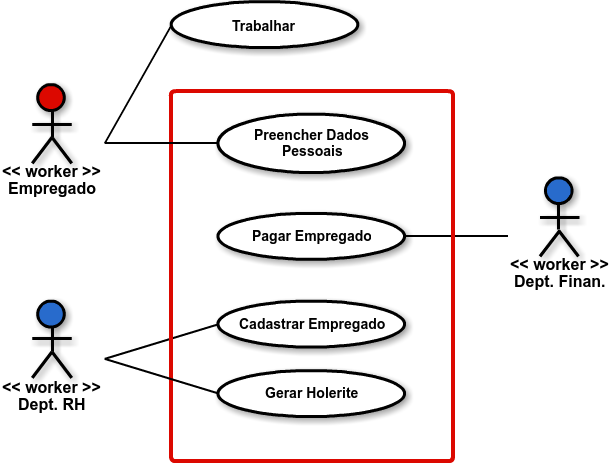
\includegraphics[width=.5\textwidth]{../Imagens/UseCaseDiagram}}
		\goodgap
		\subfigure[Atividades]{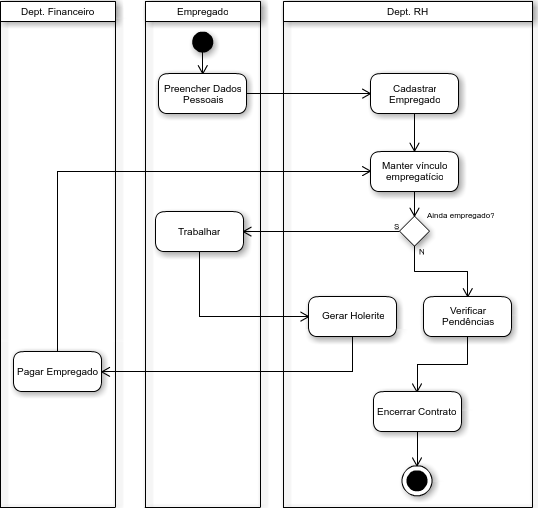
\includegraphics[width=.52\textwidth]{../Imagens/ActivityDiagram}}
		\caption{Diagramas gerados}
		\label{fig:Diagramas}
	\end{figure}
	
	\begin{figure}[h]
		\centering
		\subfigure[Máquina de Estados - Empregado]{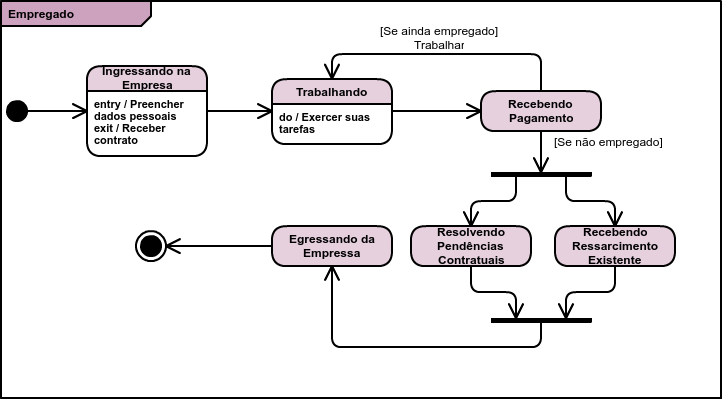
\includegraphics[width=.6\textwidth]{../Imagens/StateMachineDiagram_Empregado}}
		\goodgap
		\subfigure[Máquina de Estados - Dept. RH]{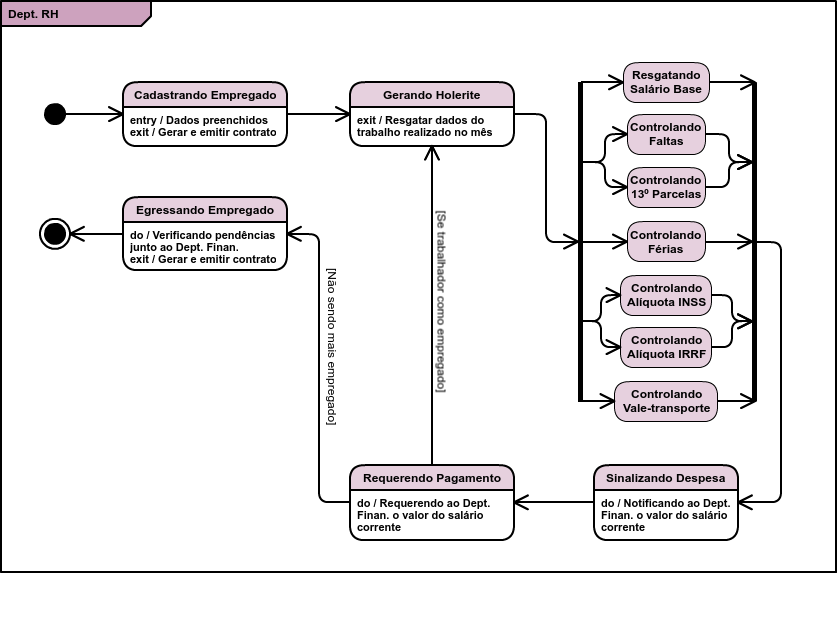
\includegraphics[width=.6\textwidth]{../Imagens/StateMachineDiagram_DeptRH}}
		\caption{Diagramas gerados, parte 2}
		\label{fig:Diagramas2}
	\end{figure}
	
	\begin{figure}[h]
		\centering
		\subfigure[Máquina de Estados - Dept. Finan.]{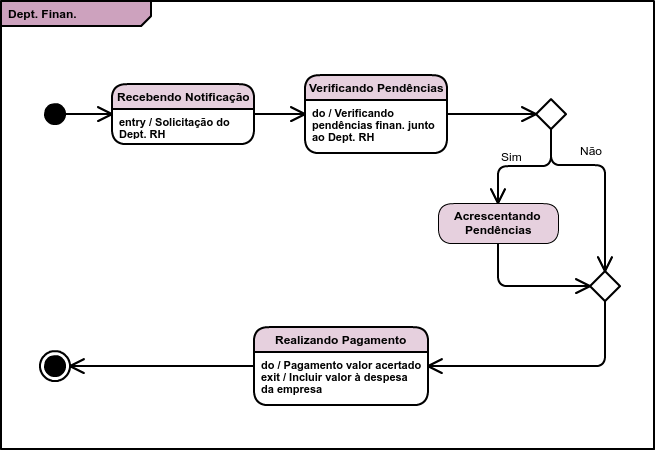
\includegraphics[width=.6\textwidth]{../Imagens/StateMachineDiagram_DeptFinan}}
		\goodgap
		\subfigure[Sequência - Preencher]{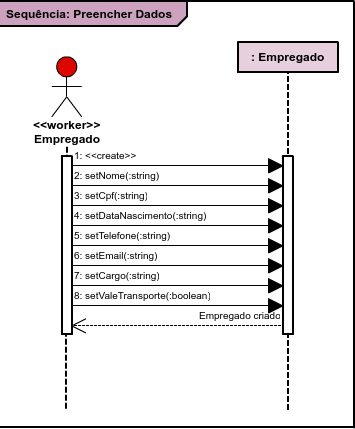
\includegraphics[width=.6\textwidth]{../Imagens/SequenceDiagram_Preencher}}
		\caption{Diagramas gerados, parte 3}
		\label{fig:Diagramas3}
	\end{figure}
	
	\begin{figure}[h]
		\centering
		\subfigure[Sequência - Cadastrar Empregado]{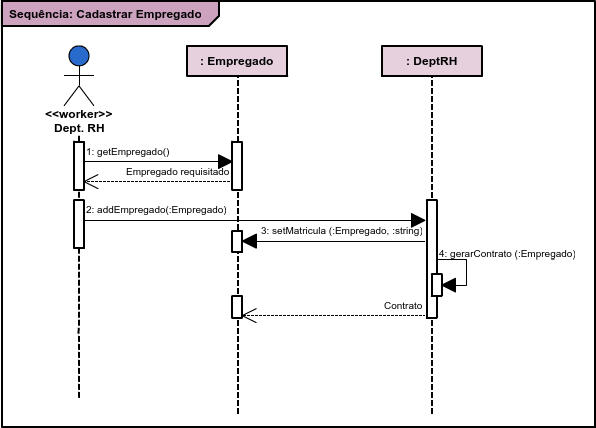
\includegraphics[width=.6\textwidth]{../Imagens/SequenceDiagram_Cadastrar}}
		\goodgap
		\subfigure[Sequência - Gerar Holerite]{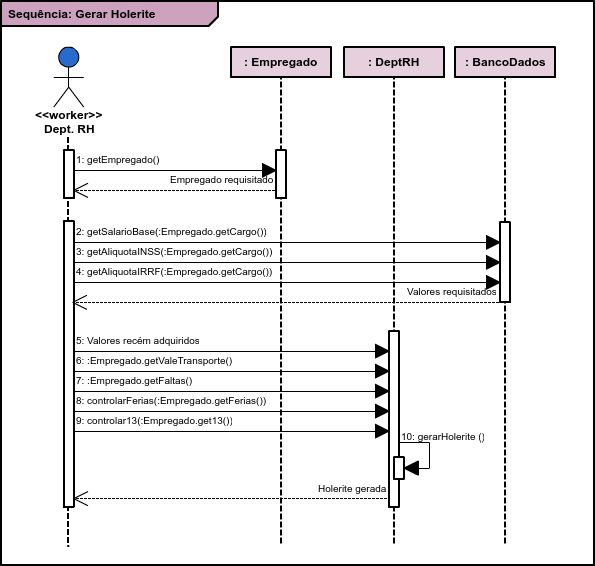
\includegraphics[width=.6\textwidth]{../Imagens/SequenceDiagram_Gerar}}
		\caption{Diagramas gerados, parte 4}
		\label{fig:Diagramas3}
	\end{figure}
	
	\begin{figure}[ht]
		\centering
		\subfigure[Sequência - Pagar Empregado]{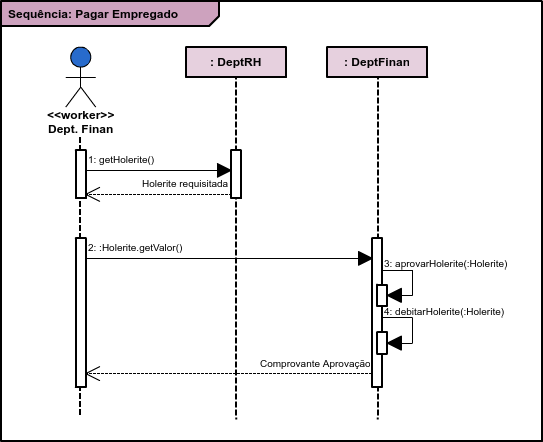
\includegraphics[width=.6\textwidth]{../Imagens/SequenceDiagram_Pagar}}
		\goodgap
		\caption{Diagramas gerados, parte 5}
		\label{fig:Diagramas4}
	\end{figure}
	

\end{document}
%%%%%%%%%%% FIM DOCUMENTO %%%%%%%%%%%%%%%%%%%%%
